\documentclass[tikz,border=8pt]{standalone}
\usetikzlibrary{arrows.meta,positioning,fit}
\begin{document}
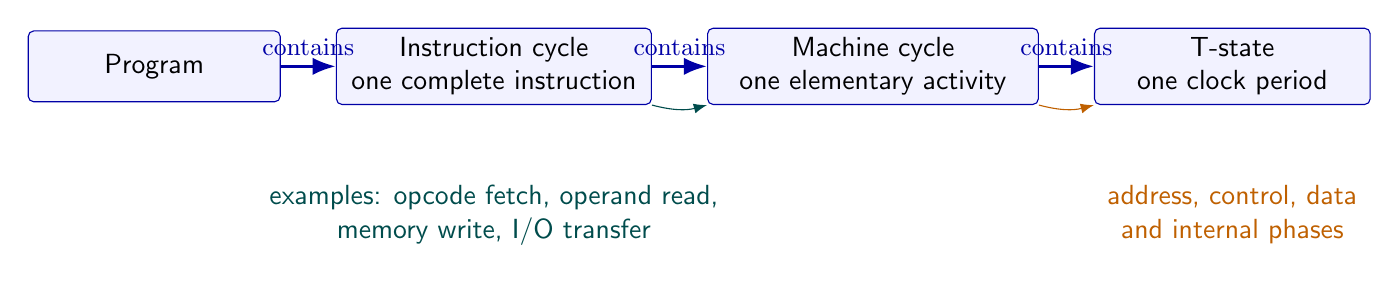
\begin{tikzpicture}[font=\sffamily,>=Latex,node distance=7mm,
box/.style={draw=blue!65!black,rounded corners=2pt,fill=blue!5,minimum height=9mm,align=center},
arr/.style={->,very thick,blue!65!black}]
\node[box,minimum width=32mm] (p) {Program};
\node[box,minimum width=40mm,right=of p] (i) {Instruction cycle\\one complete instruction};
\node[box,minimum width=42mm,right=of i] (m) {Machine cycle\\one elementary activity};
\node[box,minimum width=35mm,right=of m] (t) {T-state\\one clock period};
\draw[arr] (p)--node[above,font=\small]{contains}(i);
\draw[arr] (i)--node[above,font=\small]{contains}(m);
\draw[arr] (m)--node[above,font=\small]{contains}(t);
\node[below=9mm of i,align=center,text=teal!60!black]{examples: opcode fetch, operand read,\\memory write, I/O transfer};
\node[below=9mm of t,align=center,text=orange!75!black]{address, control, data\\and internal phases};
\draw[->,teal!60!black] (i.south east) to[bend right=15] (m.south west);
\draw[->,orange!75!black] (m.south east) to[bend right=15] (t.south west);
\end{tikzpicture}
\end{document}
